\documentclass[a4paper,fontsize = 10pt]{article}
\usepackage[nswissgerman]{babel}

% 3 column landscape layout with fewer margins
\usepackage[landscape, left=0.75cm, top=1cm, right=0.75cm, bottom=1.5cm, footskip=5pt]{geometry}
\usepackage{flowfram}
\ffvadjustfalse
\setlength{\columnsep}{1cm}
\Ncolumn{3}

%saving space around section headers and customising them
\usepackage[compact]{titlesec}  
\titlespacing{\section}{0pt}{2pt}{0pt}
\titlespacing{\subsection}{0pt}{2pt}{0pt}
\titlespacing{\subsubsection}{0pt}{2pt}{0pt}
\titleformat*{\section}{\large\bfseries}
\titleformat*{\subsection}{\normalsize\bfseries}
\titleformat*{\subsubsection}{\small\bfseries}

% define nice looking boxes
\usepackage[many]{tcolorbox}

% a base set, that is then customised
\tcbset {
  base/.style={
    boxrule=0.3mm,
    boxsep = 1mm,
    leftrule=1mm,
    left=0.5mm,
    arc=0mm, 
    fonttitle=\bfseries, 
    colbacktitle=black!10!white, 
    coltitle=black, 
    toptitle=0.0mm, 
    bottomtitle=0.0mm,
    title={#1}
  }
}

\definecolor{nicegreen}{rgb}{0.004, 0.5, 0.35}
\newtcolorbox{mainbox}[1]{
  colframe=nicegreen, 
  base={#1}
}

\newtcolorbox{subbox}[1]{
  colframe=black!20!white,
  base={#1}
}

% Mathematical typesetting & symbols
\usepackage{amsthm, mathtools, amssymb} 
\usepackage{marvosym, wasysym, dsfont}
\usepackage{derivative}
\allowdisplaybreaks

% Tables
\usepackage{tabularx, multirow}
\usepackage{booktabs}

% Make enumerations more compact
\usepackage{enumitem}
\setitemize{itemsep=0.5pt}
\setenumerate{itemsep=0.75pt}


% To include sketches & PDFs
\usepackage{graphicx}

% For hyperlinks
\usepackage{hyperref}
\hypersetup{
  colorlinks=true
}

% Metadata
\title{Cheatsheet Analysis 2}
\author{Nicolas Wehrli}
\date{January 2023}

% Math helper stuff
\def\limn{\lim_{n\to \infty}}
\def\limxo{\lim_{x\to 0}}
\def\limxi{\lim_{x\to\infty}}
\def\limxn{\lim_{x\to-\infty}}
\def\sumk{\sum_{k=1}^\infty}
\def\sumn{\sum_{n=0}^\infty}
\def\R{\mathbb{R}}
\def\C{\mathbb{C}}
\def\Q{\mathbb{Q}}
\def\N{\mathbb{N}}
\def\X{\underline{\overline{X}}}
\def\dx{\text{ d}x}
\def\P{\mathcal{P}}

\begin{document}

\maketitle

\setlength{\abovedisplayskip}{3pt}
\setlength{\belowdisplayskip}{3pt}
\setlength{\lineskip}{0pt}
\setlength{\parindent}{0pt}
\footnotesize

\section{Differential equations}
\begin{mainbox}{Ordinary Differential Equation (ODE)}
    In general an \textbf{ordinary} differential equation (ODE) relates a function $f(x)$ at $x$ to the values of its derivatives at $x$.
    I.e. it's an equation of the Form $$F(x, f(x), f'(x), f''(x), ..., f^{(n)}(x)) = 0$$ 
    The order of the diff. equation is the highest order of derivative that appears in the equation.

    A partial diff. equation is a diff. equation for a function of several variables. (It involves "partial derivatives").
\end{mainbox}
$f'(x+2) = f(x)$ is not an \textbf{ordinary} differential equation.

\begin{mainbox}{Linear ODE}
    A linear ODE of order $k$ on $I$, is an equation of the form $$y^{(k)} + a_{k-1}(x)y^{(k-1)}+...+a_1(x)y'+a_0(x)y = b(x)$$ 
    where $b, a_1, ..., a_{k-1}$ are continous functions of $x$ defined on $I$ with values in $\C$.

    If $b(x) = 0, \forall x \in I$, we call the ODE \textbf{homogeneous} and otherwise \textbf{inhomogeneous}. 
\end{mainbox}

\subsection*{Recognising a linear ODE}
\begin{itemize}
    \item no coefficients before the highest order derivative (\textbf{excluding constants})
    \item alle coefficients are continous functions
    \item no products of $y$ and it's derivatives
    \item $y$ and all of it's derivatives occur with the power one
    \item Neither $y$ nor it's derivatives are \textit{inside} another function.
\end{itemize}

\begin{mainbox}{Solutions of Linear ODE's}
    Let $I \subset \R$ open interval, $k \geq 1, k \in \N$.
    $$y^{(k)}+a_{k-1}y^{(k-1)} + ... + a_0y = b$$
    is a linear ODE over $I$ with continous coefficients.
    
    Then
    \begin{enumerate}
        \item The set of solutions $S_0$ for the associated \textbf{homogeneous} ODE (when $b = 0$), is a vector space of dimension $k$.
        \item For any initial conditions (i.e. any choice of $x_0 \in I$ and $(y_0, ..., y_{k-1}) \in \C^k$) there exists an \textbf{unique} solution $f \in S_0$ s.t. $f(x_0) = y_0, f'(x_0) = y_1, ..., f^{(k-1)}(x_0) = y_{k-1}$.
        \item For any arbitrary $b(x)$, the set of solutions of the ODE is $$S_b = \{f + f_p \mid f \in S_0\}$$ where $f_p$ is a \textbf{paritcular} solution of the ODE.
        \item For any initial condition there is a unique condition there is a unique solution $f \in S_b$.
    \end{enumerate}
     $S_b$ is \textbf{not} a Vector Space! (It's an affine Space.)
\end{mainbox}

\subsection{Linear ODE's of order 1}
$I \subset \R$ be an open interval.

We consider the diff. equation of the form \[y' + a(x)y = b(x)\]
\begin{enumerate}
  \item (Homogeneous solution) 
  \begin{align*}
    y' + a(x)y &= 0\\
    \frac{y'}{y} &= -a(x) \quad (\text{assuming } y \neq 0, \forall x \in I)\\
    \ln(|y|) &= -A(x)+C\\
    y &= e^C \cdot e^{-A(x)} = Ke^{-A(x)}, K \in \C
  \end{align*}
  If an initial condition is given, we can determine $K$.
  \item (Particular solution) 
  
  Use either ``Variation of parameters'' or ``Educated guess''.
\end{enumerate}
\subsection{Variation of parameters}
We assume that the particular solution is of the form \(f_p = K(x)e^{-A(x)}\) for a function \(K: I \to \C\). Then we can insert our guess into the ODE and see what it forces $K$ to satisfy. We get 
    \begin{align*}
        b(x) &= (K(x)e^{-A(x)})' + a(x)(K(x)e^{-A(x)})  \\
        b (x) &= K'(x)e^{-A(x)} - a(x)K(x)e^{-A(x)} + a(x)K(x)e^{-A(x)} \\
        b(x)  &= K'(x)e^{-A(x)} \\
        K'(x) &= b(x)e^{A(x)}
    \end{align*}
    and thus \[K(x) = \int_{x_0}^x b(t) e^{A(t)} \mathop{dt}\] Therefore we get \[f_p = \left(\int_{x_0}^x b(t) e^{A(t)} \mathop{dt}\right) \cdot e^{-A(t)}\]
    The method with the ``Integration factor'' gives the same particular solution!
% \subsection{Educated Guess for general case}
% \begin{enumerate}[label = (\arabic*)]
%     \item If $b(x) = x^de^{\beta x}$ and $\beta$ \textbf{is not a root of the companion Polynomial $P$}, then we try $f_p(x) = Q(x)e^{\beta x}$, where $Q$ is a Polynomial of degree $d$.
%     \item If $b(x) = x^d\cos(\beta x)$ or $b(x) = x^d\sin(\beta x)$ and $\beta$ \textbf{is not a root of the companion Polynomial $P$}, we try \[f_p(x) = Q_1(x)\cos(\beta x) + Q_2(x)\sin(\beta x)\] where $Q_1, Q_2$ are polynomials of degree $d$.
%     \item If $b$ is of the form of the previous two examples but $\beta$ \textbf{is a root with multiplicity $j$ of the companion polynomial}, then one tries the same functions, except that the Polynomials $Q$ (or $Q_1, Q_2$ resp.) have degree $d+j$.
%     \item The special case $\beta = 0$ in cases $(1), (2), (3)$ corresponds to the situation where $b$ is a polynomial of degree $d$. Therefore we try $f_p$ as a polynomial of degree $d$, unless $0$ is a root with multiplicity $j$, then we try $f_p$ as a polynomial of degree $d+j$.
% \end{enumerate}


\subsection{Educated Guess for constant coefficients}

If $b(x)$ is of a specific form, we try following $f_p$, where we insert the $f_p$ into the ODE, which gives us a system of equations for the constants:

\begin{center}
  \renewcommand*{\arraystretch}{1.6}
  \begin{tabular}{cc} 
    \toprule
    $b(x)$ & Ansatz \\ 
    \midrule
    $a \cdot e^{\alpha x}$ & $b \cdot e^{\alpha x}$\\
    $a \sin(\beta x)$ & $c \sin(\beta x) + d \cos(\beta x)$\\
    $b \cos(\beta x)$ & $c \sin(\beta x) + d \cos(\beta x)$\\
    $a e^{\alpha x} \sin(\beta x)$ & $e^{\alpha x} \Big( c \sin(\beta x) + d \cos(\beta x) \Big)$\\
    $b e^{\alpha x} \cos(\beta x)$ & $e^{\alpha x} \Big( c \sin(\beta x) + d \cos(\beta x) \Big)$\\
    $P_n(x) \cdot e^{\alpha x}$ & $R_n(x) \cdot e^{\alpha x}$\\
    $P_n(x) \cdot e^{\alpha x} \sin(\beta x)$ & $e^{\alpha x} \left( R_n(x) \sin(\beta x) + S_n(x) \cos(\beta x) \right)$\\
    $P_n(x) \cdot e^{\alpha x} \cos(\beta x)$ & $e^{\alpha x} \left( R_n(x) \sin(\beta x) + S_n(x) \cos(\beta x) \right)$\\
    \bottomrule
  \end{tabular}
\end{center}

\(P_n, R_n \) and \(S_n\) are Polynomials of degree $n$. 

\begin{enumerate}
  \item If \(b(x)\) is a linear combination of any of the base functions, try that linear combination of 'Ansatz' functions.  
  \item If $\alpha/\beta$ from any of the 'Ansatz' functions is a root of the companion Polynomial of the ODE with multiplicity $j$, then we try the same 'Ansatz' as shown in the table but multiply it with a Polynomial of degree $j$.
\end{enumerate}

\subsection{Linear ODE's with constant coefficients}
We consider an ODE of the form
\[y^{(k)} + a_{k-1} y^{(k-1)} + \ldots + a_1 y' + a_0 y = b(x)\]
We search for a homogeneous solution of the form \(e^{\lambda x}\). Now we can solve the characteristic polynomial:
\begin{align*}
  P(\lambda) = e^{\lambda x} \left(\lambda^k + a_{k-1}\lambda^{k-1} + \ldots + a_0\right) = 0 \\ 
  \implies 0 = \lambda^k + a_{k-1}\lambda^{k-1} + \ldots+ a_0
\end{align*}
\begin{itemize}
    \item The roots of \(P(\lambda)\) are the Eigenvalues \(\lambda_i\), with corresponding multiplicity \(m_r\). Thus the functions \(f_{i,r} : x \to x^r e^{\lambda_i x}, 0 \leq r < m_r\) span the Vector Space \(S_0\).
    \item If \(\lambda = \beta + \gamma i\) is a complex of \(P(\lambda)\), then the complex conjugation, i.e. \(\bar{\lambda} = \beta - \gamma i\) is also a root. Thus \(f_1 = e^{\lambda x}\) and \(f_2 = e^{\bar{\lambda} x}\) are solutions to the homogeneous equation.
    \item We realize that \(f_1 = e^{\lambda x} = e^{\beta x} (\cos(\gamma x)+ i \sin(\gamma x))\) and \(f_2 = e^{\bar{\lambda} x}= e^{\beta x} (\cos(\gamma x) - i \sin(\gamma x))\).
    \item We can thus replace $f_1$ and $f_2$ by \(\tilde{f_1} = e^{\beta x} \cos(\gamma x)\) and \(\tilde{f_2} = e^{\beta x} \sin(\gamma x)\). (Note that $f_1 = \tilde{f_1} + i \tilde{f_2}$ and $f_2 = \tilde{f_1} - i \tilde{f_2}$)
    \item Note that we are often only interested in finding real-valued solutions if the coefficients are all real valued.
    \item If \(y^{(k)} + a_{k-1}y^{(k-1)} + \dots + a_0 y = 0\) only has real coefficients, every pair of complex conjugated roots $\beta_j \pm \gamma_j i$ with multiplicity $m_j$ leads to a solution \[x^l e^{\beta_j x} \Big( \cos(\gamma_j x) \pm i \sin(\gamma_j x) \Big) \quad \text{for }0 \leq l < m_j\]
    of which then the real part can be extracted.
\end{itemize}
To find a particular solution $f_p$ we can as in the general case use \textbf{Varation of parameters} or \textbf{Educated guess}. We will now show an simple example with $2$ basis functions:

Consider the Linear ODE $y'' + y a_1y' + a_0y = b$
\begin{enumerate}[label=(\arabic*)]
  \item Assume the space of homogeneous solutions $S_0$ is spanned by $f_1, f_2$, i.e. $f_0 = f_1 + f_2$ is also a solution  
  \item Now we try \(f_p = z_1(x) f_1 + z_2(x) f_2\)
  \item We first insert $f_p$ into the ODE and we require the additional constraint that $ z_1'(x) f_1 + z_2'(x) f_2 = 0$ to find a concrete solution. 
  
  Therefore we get the following system of equations:
  \begin{align*}
    z_1'(x) f_1 + z_2'(x) f_2 &= 0\\
    z_1'(x) f_1' + z_2'(x) f_2' &= b(x)\\
  \end{align*}
  We can solve this as follows:
  \begin{align*}
    W &= f_1 f_2' - f_2 f_1' \neq 0\\
    \Rightarrow z_1' &= \frac{-f_2 b}{W} \; , z_2' = \frac{f_1 b}{W}\\
    \Rightarrow f_p &= \left(\int \frac{-f_2 b}{W} dt\right)f_1  + \left(\int \frac{f_1 b}{W} dt\right)f_2 
  \end{align*}
\end{enumerate}

\subsection{Seperation of Variables}
    Consider a differential equation of the form 
    \begin{align*}
        y'(x) &= b(x)g(y)
    \end{align*}
    Assume $g(y(x)) \neq 0$. If $\exists y_0$ s.t. $g(y_0(x)) = 0$ then $y = y_0$ is a solution.
    \begin{align*}
        \frac{y'(x)}{g(y(x))} &= b(x)\\
        \int \frac{y'(x)}{g(y(x))} \mathop{dx} &= \int b(x) \mathop{dx}\\
    \end{align*}
    Applying substitution with $u = y(x)$ we obtain 
    $$\int \frac{1}{g(u)}\mathop{du} = \int b(x) \mathop{dx}$$
    We can then determine both integrals and solve for $u = y$.

\section{Derivations in \texorpdfstring{\(\R^n\)}{Rⁿ}}
\begin{subbox}{Monomial in $\R^n$}
  A Monomial of degree \(e\) is a function $f: \R^n \mapsto \R:$
  \begin{align*}
    (x_1, \ldots, x_n) \mapsto \alpha x_1^{d_1}\cdot \ldots \cdot x_n^{d_n} \\
    e = d_1 + \ldots + d_n 
  \end{align*}
  \(\to\) i.e. a Polynomial that only has one term.
\end{subbox}
\begin{mainbox}{Polynomial in $\R^n$}
  A Polynomial with \(n\) variables of degree \(d\) is a finite sum of Monomials of degree \(e \le d\).
\end{mainbox}

\subsection{Convergence}
\begin{enumerate}
  \item Dot product: \(\left< x,y\right> = \sum_{i=0} x_i \cdot y_i\)
  \item Euclidean norm: \(||x|| := \sqrt{x_2^1 + \cdots + x_n^2}\) with the following properties:
  \begin{enumerate}
    \item \(||x|| \ge 0, ||x|| = 0 \iff x = 0\)
    \item \(||\lambda x|| = |\lambda| \cdot ||x||, \forall \lambda \in \R\)
    \item \(||x+y|| \le ||x|| + ||y||\)
    \item \(|\left<x,y\right>| \le ||x|| \cdot ||y||\)
  \end{enumerate}
\end{enumerate}

\begin{mainbox}{Definition Convergence}
  Let \((x_k)_{k \in \mathbb{N}}, x_k \in \R^n\). The following definitions for \(\lim_{k\to\infty}x_k = y\) equivalent:
  \begin{enumerate}
    \item \(\forall \epsilon > 0 \exists N \ge 1\) such that \(\forall k \ge N \ ||x_k - y|| < \epsilon\).
    \item For every \(i, 1 \le i \le n\) the sequence \((x_{k,i})_k\) of real numbers converges to \(y_i\).
    \item The sequence \(||x_k - y||\) of real numbers converges to \(0\).
  \end{enumerate}
\end{mainbox}
\subsection{Continuity}
\begin{mainbox}{Definition Continuity}
    Let \(f: \X \subset \R^n \to \R^m\)  and \(x_0 \in \X\). 
    
    \(f\) is continous in \(x_0\), if one of the following conditions is fulfilled:
    \begin{enumerate}
        \item \(\forall \epsilon > 0 \ \exists \delta > 0\) such that for all \(x \in \X\) \[||x - x_0|| < \delta \implies ||f(x) - f(x_0)|| < \epsilon\]
        \item \(\forall\) sequences \((x_k)\) in \(X\) with \(\lim_{k \to \infty} x_k = x_0\) we have \[\lim_{k \to \infty} f(x_k) = f\left(\lim_{k \to \infty} x_k\right) = f(x_0)\]
    \end{enumerate}
\end{mainbox}
\(f\) is continous on \(\X\) $\iff$ \(f\) is continous at every point \(x_0 \in \X\). 

In Addition we have the following:
\begin{enumerate}
  \item Cartesian product of continous functions is continous.
  \item \(f: \R^n \mapsto \R^m\)\\
  \((x_1, \ldots, x_n) \mapsto (f_1(x),\ldots,f_m(x))\) \\is continous $\iff$ \(f_i: \R^n \to \R\) continous \(\forall i = 1, \ldots, m\).
  \item Linear Maps \(x \mapsto Ax\) are continous.
  \item Finite sums and products of continous functions are continous.
  \item Functions with seperated Variables are continous if each factor is continous. (i.e. $f(x_1,...,x_n) = f_1(x_1)f_2(x_2)\cdot...\cdot f_n(x_n)$ is continous if $f_1, f_2, ..., f_n$ are continous.)
  \item In particular Polynomials are continous.
  \item The composition of continous functions is continous.
  \item If $f: \R^2 \mapsto \R$ is continous. For an arbitrary fixed $y_0 \in \R$ we can define $g_{y_0}(x) := f(x, y_0)$. Since $g_{y_0}$ is a composition of continous functions it is also continous. 
  \item Warning! The converse is not true. $g_{y_0}$ continous for all $y_0 \in \R$ does \textbf{not} imply that  $f$ is continous!
\end{enumerate}
\begin{mainbox}{Sandwich-Lemma}
  If \(f, g, h: \R^n \to \R\) are functions with \(f(x) < g(x) < h(x) \\ \forall x \in \R^n\). Let $a \in \R^n$:
  \[\lim_{x\to a} f(x) = \lim_{x \to a} h(x) = L \implies \lim_{x\to a} g(x) = L\]
\end{mainbox}
\subsection{Properties of sets}
A set \(\X \subset \R^n \) is
\begin{itemize}
  \item \textbf{bounded}, if the set \(\{ ||x|| \mid x \in \X \}\) is bounded in \(\R\)(i.e. \(\exists K \ge 0, \forall x \in \X: ||x|| \le K\)).
  \item \textbf{closed}, if every sequence \((x_k)_{k\in \N} \subset \X\), that converges to some Vector \(y \in \R^n\), we have \(y \in \X\) (i.e. limits of sequences in $X$ are also in $X$).
  \item \textbf{compact}, if its closed and bounded.
  \item \textbf{open} if, for any $x =(x_1,x_2,...,x_n) \in \X$, there exists $\delta >0$ such that the set \[\{y = (y_1,...,y_n) \in \R^n \mid |x_i-y_i|< \delta, \forall 1 \leq i \leq n\}\] is contained in $\X$.
  \item \textbf{convex}, if \(\forall x, y \in \X: \lambda x + (1 - \lambda)y \in \X, \forall 0 \leq \lambda \leq 1\) (the line segment between \(x, y\) is contained in \(\X\)).
  \item \textbf{open}, if and only if the complement $Y = \R^n \setminus \X$ is \textbf{closed}. (Equivalent definition)
\end{itemize}
\textbf{Important examples:}
\begin{itemize}
  \item \((a,b) \subset \R\) is open.
  \item \(\left[a,b\right) \subset \R\) is neither open nor closed.
  \item \(\R^n\) and \(\emptyset\) are both open and closed. There exists no other set in $\R^n$ which is both open and closed.
  \item If $X \subseteq \R^n, Y \subseteq \R^m$ are both bounded (rsp. closed/compact) then $X \times Y \subseteq \R^{n+m}$ is bounded (rsp. closed/compact)
  \item In particular the cartesian product of compact intervals $I_i \in \R$: $I_1 \times I_2 \times ... \times I_n = \{(x_1,x_2,...,x_n) \in \R^n \mid x_i \in I_i\}$ is compact (i.e. closed and bounded).
  \item Let $f: \R^n \mapsto \R^m$ be continous. Then for every closed(/open) set $Y \subseteq \R^m$, the set $f^{-1}(Y)$ is closed(/open). 
\end{itemize}
\begin{subbox}{Bolzano-Weierstrass}
  Every bounded sequence in \(\R^n\) has a converging partial sequence.
\end{subbox}
\begin{subbox}{Min-Max-Theorem}
  Let \(\X \subset \R^n, \X \ne \emptyset\) be compact and \(f: \X \to \R\) a continous function. Then \(f\) is bounded and achieves a max and a min. I.e. $\exists x^+,x^- \in \X$, such that
  \[f(x^+) = \sup_{x\in \X} f(x) \quad f(x^-) = \inf_{x \in \X} f(x)\]
\end{subbox}

\subsection{Partial Derivatives}
\begin{mainbox}{Partial Derivative}
    To find the partial derivative of \(f: \X \subset \R^n \to \R\) (whereby \(\X\) open) with respect to $x_j, 1 \leq j \leq n$ at a point $x_0 \in \X$ we define:
\[\partial_j f (x_0)= \pdv{f}{x_{j}}(x_0) = \lim_{h \to 0} \frac{f(x_0 + h\cdot e_j) - f(x_0)}{h}\]where $e_j$ is the $j$-th canonical basis vector of $\R^n$.
\end{mainbox}
 
For \(f: \R^n \to \R^m, x_0 \in \R^n\) we have
\begin{align*}
  \pdv{f(x_0)}{x_j} := \begin{pmatrix}
    \pdv*{f_1(x_0)}{x_j}\\
    \vdots\\
    \pdv*{f_m(x_0)}{x_j}\\
  \end{pmatrix}
\end{align*}
Partial derivatives have following properties:
\begin{enumerate}
  \item \(\partial_j(f + g) = \partial_j (f) + \partial_j g\)
  \item \(\partial_j(f \cdot g) = \partial_j (f) \cdot g + \partial_j (g) \cdot f\)
  \item \(\partial_j(f / g) = \frac{\partial_j (f) \cdot g - \partial_j (g) \cdot f}{g^2}\) for \(g \ne 0\)
\end{enumerate}
\begin{mainbox}{Jacobi-Matrix}
Let \(f: \X \subset \R^n \to \R^m\) and \(\X\) an open set. The Jacobi-Matrix is the \(m \times n\) Matrix:
\[J_f = \left( \pdv{f_i}{x_j} \right)_{\substack{1 \leq j \leq n \\ 1 \leq i \leq m}}\]
\end{mainbox}
\begin{mainbox}{Gradient}
    In the special case of a function \(f: \X \subset \R^n \to \R\), the Jacobi-Matrix is a row vector which transposed gives us \(\nabla f\). The geometric interpretation is a vectorfield, defined by $\nabla f$, which indicates the direction and magnitude of the biggest growth of $f$. 
\end{mainbox}

% \begin{subbox}{Divergenz}
%   Die Divergenz einer Funktion \(f\) ist die Spur der Jacobi-Matrix von \(f\). \[\text{div}(f)(x_0) = \text{Tr}(J_f(x_0)) = \sum_{i=0}(J_f)_{i,i}\]
% \end{subbox}

\subsection{Differentiability}
\begin{mainbox}{Differentiability}
    Let $\X \subset \R^n$ be open, $x_0 \in \X$. We have 
    $f: \X \to \R^m$. 

    We say that $f$ is \textbf{differentiable} at $x_0$, with the differential $u$, if there exists a \textbf{linear map} $u: \R^n \to \R^m$ such that 
    \[\lim_{\substack{x \to x_0 \\ x \neq x_0}} \frac{f(x)-f(x_0)-u\cdot(x-x_0)}{||x-x_0||} = 0\]
    We denote $u = df(x_0) = d_{x_0}f$.
\end{mainbox}
\begin{itemize}
    \item If $f$ is differentiable at all points $x_0 \in \X$, then $f$ is differentiable on $\X$.
    \item Having all partial derivatives defined is not sufficient to conclude Differentiability.
    \item If all partial derivatives are defined and continous, then $f$ is differentiable.
\end{itemize}
\begin{mainbox}{Conclusions from Differentiability}
    If \(f,g\) are differentiable in \(x_0 \in \X\) we have:
    \begin{enumerate}
    \item \(f\) is continous in \(x_0\)
    \item \(f\) has all partial derivatives at \(x_0\) and the matrix of the linear map \(df(x_0): x \mapsto Ax\) is given by the \textbf{Jacobi-Matrix} of \(f\) at \(x_0\), i.e. \(A = J_f(x_0)\)
    \item \(d(f+g)(x_0) = df(x_0) + dg(x_0)\)
    \item If \(m = 1\), then \(f\cdot g\) is differentiable. If additionally \(g \ne 0\), then \(f/g\) is also differentiable. (Product rule and Quotient rule apply)
    \item (Chain rule): Let $\X \subseteq \R^n, Y \subseteq \R^m$ be open. 
    
    If \(f: \X \to Y, g: Y \to \R^p\) are both differentiable, we have \(d(g \circ f)(x_0) = dg(f(x_0)) \circ df(x_0)\). 
    Furthermore \[J_{g \circ f}(x_0) = J_g(f(x_0)) \cdot J_f(x_0)\]
    Therefore \[d(g \circ f)(x_0): \X \to \R^p \qquad x \mapsto J_g(f(x_0)) \cdot J_f(x_0) \cdot x\]
    \end{enumerate}
\end{mainbox}

\begin{subbox}{Tangent Space}
  The \textbf{tangent space} at $x_0$ of \(f\) is given by the graph of the affine linear map \(g(x) = f(x_0) + df(x_0)(x-x_0)\).
  
  I.e. \[\{(x,g(x)) \in \R^n\times\R^m \mid g(x) = f(x_0) + df(x_0)(x-x_0)\}\]
\end{subbox}

\begin{subbox}{Directional Derivative}
    Let $f: \X \subseteq \R^n \to \R^m$ be differentiable at $x_0 \in \X$.
    For any $v \in \R^n, v \neq 0$ the \textbf{directional Derivative} of $f$ at $x_0$ exists and is defined as 
    \[\partial_v f(x_0) = \lim_{h \to 0} \frac{f(x_0 + hv)-f(x_0)}{h} = J_f(x_0) \cdot v\] 
\end{subbox}
\begin{mainbox}{Change of variables (Bijection)}
    Let $\X \subset \R^n$ be open and $f: \X \to \R^n$ differentiable. $f$ is a \textbf{change of variable} around $x_0 \in \X$ if there exists a radius $r > 0$ such that the Ball 
    \[B_r(x_0) := \{x \in \R^n \mid ||x-x_0|| < r\}\] 
    has the property that the Image $Y = f(B_r(x_0))$ is open and there exists a differentiable map $g: Y \to B_r(x_0)$ such that $f \circ g = g \circ f =\text{id}$.

    We find that if det\((J_f(x_0)) \neq 0\) (i.e. $J_f(x_0)$ is invertible), then $f$ is a change of variables around $x_0$. Moreover the Jacobian of the inverse map $g$ is determined by \[J_g(f(x_0)) = J_f(x_0)^{-1}\]
    (Analog to the fact that a function $h: I \subseteq \R \to \R$ is bijective from $I$ to its image if $h' > 0$ or $h' < 0$)
\end{mainbox}
\subsection{Higher derivatives}
\subsubsection*{Notation for higher partial derivatives}
    
For a function $f: \R^n \to \R^t$ we denote higher order partial derivatives with the following:

    First let $m = (m_1, m_2, ..., m_n)$ and $|m| = m_1 + m_2 + ... + m_n$.

    We write
    \[\frac{\partial^{|m|}f_j}{\partial x_1^{m_1} \partial x_2^{m_2} \cdot ... \cdot \partial x_n^{m_n}} = \partial_{x^m}^{|m|}f_j, \ 1 \leq j \leq t\]


\subsubsection*{Differential Classes}
    Let \(\X \subset \R^n\) be open, $f : \X \to \R^m$. 
    \begin{itemize}
        \item We say that $f$ is differentiable of class $C^1$ if $f$ is differentiable on $\X$ and all its partial derivatives are continous. The set of all $C^1$ functions from $\X$ to $\R^m$ are denoted by $C^1(\X:\R^m)$.
        \item Let $k \geq 2$. We say $f \in C^k(\X:\R^m)$ (i.e. $f$ is of class $C^k$) if its differentiable and each $\partial_{x_i}f: \X \to \R^m$ ($1 \leq i \leq n$) is of class $C^{k-1}$.
        \item We say that $f$ is smooth or of class $C^\infty$ if $f \in C^k, \ \forall k \in \N$.
        \item All polynomials, trigonometric and exponential functions are of class $C^\infty$.
        \item If $f \in C^k, k \geq 2$ then all partial derivatives of order $\leq k$ are commutative.
        $$\pdv{f}{x_i, x_j} = \pdv{f}{ x_j, x_i}$$
    \end{itemize}

\begin{mainbox}{Hessian}
    Let $\X \subset \R^n$ be open and $f: \X \to \R$ a $C^2$ function.

    For an $x_0 \in \X$, the \textbf{Hessian matrix} of $f$ at $x_0$ is the symmetric \(n \times n\) matrix that denotes the second derivative:
    \[\text{Hess}_f(x_0) := \left(\pdv{f(x_0)}{x_i, x_j}\right)_{1\le i,j \le n}\] 
    Sometimes we also denote it by $\nabla^2f(x_0)$ or $H_f(x_0)$.
\end{mainbox}
\subsection{Taylor polynomials}
Let \(k \le 1\) and \(f: \X \mapsto \R\) be a funciton of class \(C^k\) on \(\X\), and fix \(x_0 \in \X\). The \(k\)-th Taylor polynomial of \(f\) at the point \(x_0\) is the polynomial in \(n\) variables of degree \(\le k\) given by
\begin{align*}
  &T_k f(y; x_0) = f(x_0) + \sum_{i=1}^n \partial_i f(x_0) \cdot y_i + \dots \\
  &+ \sum_{m_1 + \cdots + m_n = k} \frac{1}{m_1! \cdots m_n!} \pdv{^k f(x_0) }{x_1^{m_1} \cdots \partial x_n^{m_n}} \cdot y_1^{m_1} \cdots y_n^{m_n}
\end{align*}
Using our new notation for higher-order derivatives we can denote the Taylor polynomial by
\[T_k(y; x_0) = \sum_{|m| \leq k} \frac{1}{m!}\partial_{x^m}^{|m|}f(x_0)\cdot y^m\]
with $m! = m_1!m_2!\cdot ... \cdot m_n!$

\subsubsection*{Examples}
\begin{align*}
  T_1 f(\vec{x}; x_0) &:= f(x_0) + \nabla f(x_0) \cdot \vec{x} \\
  T_2 f(\vec{x}; x_0) &:= T_1f + \frac{1}{2} \cdot \vec{x}^\top \cdot \text{Hess}_f(x_0) \cdot \vec{x}
\end{align*}


\subsection{Extrema}
\subsubsection*{Local Extrema}
Let \(f: \X \subset \R^n \mapsto \R\) be differentiable and \(\X\) open. 

Then \(x_0 \in \X\) is a \textbf{local Maximum (Minimum)} if there exists an $r > 0, r \in \R$ and \(B_{x_0}(r) = \{x\in \R^n \mid ||x-x_0|| < r \} \subset \X\) such that:
\[\forall x \in B_{x_0}(r): f(x) \le (\ge) f(x_0)\]
If \(x_0 \in \X\) is a local extrema, we additionally have \(\nabla f(x_0) = 0\).

\subsubsection*{Critical point}
A point \(x_0 \in \X\) with \(\nabla f(x_0) = 0\) is a \textbf{critical point}. 

Critical points are candidates for local extrema.

If additionally \(\det(\text{Hess}_f(x_0)) \ne 0\), then \(x_0\) is a \textbf{non-degenerate} critical point.

\subsubsection*{Saddle point}
If a critical point is neither a maximum nor a minimum, we call it a \textbf{saddle point}.

\subsubsection*{Global Extrema}
Let \(f: K \mapsto \R\) and \(K\) compact, then a global extrema of \(f\) exists and is either at a point $x_0$ in the interior of \(K\) or on the boundary of $K$. To determine such an global extrema we split \(K\) into it's interior \(\X\) and the boundary \(B\). 

First we determine the critical points of \(\X\). To determine the Maximas/Minimas \(B\), we will need Knowledge from Analysis I (redefine the boundary as a union of sets dependend on 1 variable, i.e. Linesegments).
\subsubsection*{Testing critical points}
Let \(f: \X \subseteq \R^n \mapsto \R, \X\) open and \(f\in C^2\). Let \(x_0\) be a \textbf{non-degenerate critical point} of \(f\). Then we:
\begin{enumerate}
  \item $\text{Hess}_f(x_0)$ pos. def. \(\implies\) $x_0$ is a local Minimum.
  \item $\text{Hess}_f(x_0)$ neg. def. \(\implies\) $x_0$ is a local Maximum.
  \item $\text{Hess}_f(x_0)$ indefinite \(\implies\) $x_0$ is a saddle point.
\end{enumerate}
If \(x_0\) is a \textbf{degenerate critical point}, we can't conclude anything in general. In such a case we would have to verify the signs in the neighborhood of $x_0$. (Not much information found on how to do that in multi-variable calculus)
\subsubsection*{Critical points with constraints}
If we want to determine the Minimas/Maximas of a function \(f: \X \mapsto \R\) with the constraint \(g(x) = 0, g: \X \mapsto \R\), we can use the Lagrange multipliers.
\begin{subbox}{Lagrange multipliers}
  Let \(\X \subset \R^n\) be open and \(f,g: \X \mapsto \R\) functions of \(C^1\). If $x_0$ is a local extremum of $f$ restricted to the set \[Y = \{x \in \X \mid g(x) = 0\}\] then either $\nabla g(x_0) = 0$, or there exists $\lambda \in \R$ such that 
     \[\nabla f(x_0) = \lambda \cdot \nabla g(x_0)\] and \(g(x_0) = 0\).
\end{subbox}

\subsection{Definite}
A symmetric (non-singular) matrix $A$, det$A \ne 0$ is
\begin{itemize}
  \item \textbf{positive definite} $\iff$ all Eigenvalues are positive $\iff$ all principal minors of $A$ are positive
  \item \textbf{negativ definite} $\iff$ all E.V. are negative $\iff$ $-A$ is positive definite.
  \item \textbf{indefinite} if it has positive and negative Eigenvalues.
\end{itemize}
Eigenvalues can be found with the characterstic polynomial:
\begin{align*}
  \text{det} \left(
  \begin{pmatrix}
    a & b\\
    c & d
  \end{pmatrix}
  -
  \begin{pmatrix}
    \lambda & 0\\
    0 & \lambda
  \end{pmatrix}
  \right)
  &=
  \text{det}
  \begin{pmatrix}
    a - \lambda & b\\
    c & d - \lambda
  \end{pmatrix}\\
  &\Rightarrow ad - (a + d) \lambda + \lambda^2 - bc = 0
\end{align*}
For non-symmetric Matrices we have to test for all Vectors \(v\), if \(v^\top A v > 0\) (rsp. \(< 0\)).
\subsubsection*{3D Determinant}
\begin{align*}
  a \cdot \text{det}
  \begin{pmatrix}
    e & f\\
    h & i
  \end{pmatrix}
  - b \cdot \text{det}
  \begin{pmatrix}
    d & f\\
    g & i
  \end{pmatrix}
  + c \cdot \text{det}
  \begin{pmatrix}
    d & e\\
    g & h
  \end{pmatrix}
\end{align*}

\begin{subbox}{Principal Minor}
    The $k$-th leading principal minor of $A$ is given by 
    \[M_k = \text{det}\left((A)_{1:k,1:k}\right)\]
\end{subbox}


\section{Integrals in \texorpdfstring{\(\R^n\)}{Rⁿ}}
\subsection{Simple Integrals}
For \(f: \R \mapsto \R^n\) we define the integral of $f$ as
\[\int_a^b f(t)dt = 
\begin{pmatrix*}
  \int_a^b f_1(t) dt \\
  \vdots\\
  \int_a^b f_n(t) dt
\end{pmatrix*}
\]

\subsection{Line Integrals (Path Integrals)}
\begin{mainbox}{A parameterized curve}
    A parameterized curve in \(\R^n\) is a continous map \(\gamma: \left[a,b\right] \mapsto \R^n\) that is piecewise in \(C^1\), 
    i.e. \(\exists k > 1, k \in \N\) and a partition \(a = t_0 < t_1 < ... < t_k = b\), such that 
    \[\gamma|_{[t_{i-1}, t_i]} \in C^1, \forall 1 \leq i \leq k.\] 
    A parameterized curve does not have to be injective.
  \end{mainbox}
  \textbf{Useful trick:}

  In general if $\gamma: [a, b] \to \R^n (t \mapsto \gamma(t))$ is a curve, then $\alpha: [a,b] \to \R^n$ with $\alpha(t) := \gamma(b+a - t)$ traces the same curve in the opposite direction. 
  
\begin{mainbox}{Line(Path) Integrals}
    Let \(\gamma : \left[a,b\right] \mapsto \R^n\) be a parameterized curve and \(\X \subset \R^n\) a set containing the image of $\gamma$, and let $f: \X \to \R^n$ be a continous function. The \textbf{Line Integral (Path Integral)} is defined as 
    \[\int_\gamma f(s) \mathop{ds} = \int_a^b f(\gamma(t)) \cdot \gamma'(t) \mathop{dt}\]
    For Notation $s$ represents $\gamma(t)$ and $\mathop{ds}$ represents $\gamma'(t)\mathop{dt}$.
\end{mainbox}

Line Integrals have following properties:
\begin{enumerate}
  \item It is independent of orientation preserving reparameterization of the curve:
  \begin{align*}
    \gamma&: [a,\, b] \mapsto \R^n\\
    \sigma&: [c, \, d] \mapsto [a, \, b], \ \sigma'(t) > 0 \ \forall t \in (c, \ d)\\
    \tilde{\gamma}&: [c,\, d] \mapsto \R^n\\
    \tilde{\gamma} &= \gamma \circ \sigma = \gamma(\sigma)\\
    \Rightarrow &\int_\gamma f(s) \; ds = \int_{\tilde{\gamma}} f(s) \; ds
  \end{align*}
  \item We have $\gamma_1: [a, \ b] \to \X \subset \R^n, \gamma_2: [c, \ d] \to \X$ with $\gamma_1(b) = \gamma_2(c)$. We can now concatenate these 2 curves to \(\gamma_1 + \gamma_2\) 
  \begin{align*}
    \gamma_1 + \gamma_2 &:=
    \begin{cases}
      \gamma_1(t) \quad& t \in [a, \, b]\\
      \gamma_2(t - b + c) \quad& t \in [b, \, b+ (d - c)]
    \end{cases}\\
    \int_{\gamma_1 + \gamma_2} f(s) \; ds &= \int_{\gamma_1} f(s) \; ds + \int_{\gamma_2} f(s)\; ds
  \end{align*}
  \item Let \(\gamma : \left[a,b\right] \mapsto \R^n\) be a path and \(-\gamma: [a, b] \to \R^n\) the same path in the opposite direction (i.e. \((-\gamma)(t) = \gamma(a + b - t)\)). Then we have
  \[\int_{-\gamma} f(s)ds = -\int_\gamma f(s) ds\]
\end{enumerate}

\subsection{Potential}
A differentiable function \(g: \X \subset \R^n \mapsto \R\) with \(\nabla g = f, f: \X \mapsto \R^n\) is called a \textbf{potential} for \(f\). This can be used as follows:
\begin{align*}
  \int_\gamma f \; ds &= \int_a^b f(\gamma(t)) \cdot \gamma'(t) \; dt\\
  &= \int_a^b \nabla g(\gamma(t)) \cdot \gamma'(t) \; dt\\
  &= \int_a^b \frac{d}{dt} (g \circ \gamma) \; dt\\
  &= (g \circ \gamma)(b) - (g \circ \gamma)(a)
\end{align*}
For a function $f: \R^n \to \R^n$ there is not always a potential $g$! And continuity of $f$ is not sufficient for the existence of a potential for $f$. (Counterexample: $f(x,y) = (2xy^2,2x)$)
\subsection{Conservative Vector fields}
\begin{subbox}{Conservative Vector fields}
    $f: \X \to \R^n$ continous Vector field. If for any $x_1, x_2 \in \X$ the line integrals $\int_{\gamma}f \mathop{ds}$ for any curve between $x_1,x_2$ are equal, $f$ is called \textbf{conservative}.
\end{subbox}

Let \(\X\) be open and a path-connected subset of $\R^n$. Let \(f: \X \subset \R^n \mapsto \R^n\) be a continous vector field. The following are equivalent:
\begin{enumerate}
  \item $f$ is the gradient of a function $g: \X \to \R$, i.e. $f = \nabla g$.
  \item The line integral of $f$ is independent of the path between any 2 points.
  \item The line integral of $f$ along any closed path is always $0$. (A closed path $\gamma: [a, b] \to \X$ fulfills $\gamma(a) =\gamma(b)$)
\end{enumerate}
We additionally have this necessary but not sufficient condition:
\[f \text{ is conservative }\implies \pdv{f_i}{x_j} = \pdv{f_j}{x_i} \quad \forall i,\, j\]

\begin{subbox}{Path-connected set}
  Let \(\X \subset \R^n\) be open. \(\X\) is path-connected, if for every pair of points \(x, y \in \X\) there exists a parameterized curve \(\gamma : \left[0, 1\right] \mapsto \X\), such that \(\gamma(0) = x, \gamma(1) = y\).
\end{subbox}

\begin{subbox}{Starshaped set}
  A subset \(\X \subset \R^n\) is starshaped if there \(\exists x_0 \in \X\) such that, \(\forall x \in \X\) the line segment joining \(x_0\) to \(x\) is contained in \(\X\). 
  \[\X \text{ convex} \implies \X \text{ starshaped}\]
\end{subbox}
If \(\X\) is a starshaped, open subset of \(\R^n\) and \(f \in C^1\) a vector field, we have:
\begin{align*}
    \pdv{f_i}{x_j} = \pdv{f_j}{x_i} \quad \forall i,\, j
  \quad &\Rightarrow \quad \text{$f$ is conservative}\\
  \text{For $f: \X \subset \R^3 \to \R^3, f \in C^1$ we also have: }\\
  \text{curl}(f) = \begin{pmatrix}
    0\\0\\0
  \end{pmatrix}
  \quad &\Rightarrow \quad \text{$f$ is conservative}
\end{align*}
(As above only for $f: \X \subset \R^3 \to \R^3$) 
\\\(\text{curl}(f)\) is defined as
\[\text{curl}(f) := \begin{pmatrix}
  \partial_y f_3 - \partial_z f_2 \\
  \partial_z f_1 - \partial_x f_3 \\
  \partial_x f_2 - \partial_y f_1
\end{pmatrix}\]
\subsection{Riemann Integral in \texorpdfstring{\(\R^n\)}{Rⁿ}}
\begin{subbox}{Cuboid / box in $\R^n$}
    A \textbf{cuboid} or box $Q \subset \R^n$ is a set of the form
    $$Q = [a_1, b_1] \times [a_2,b_2] \times ... \times [a_n,b_n], \quad a_k, b_k \in \R$$
    The \textbf{volume function} vol($\cdot$) assigns to each cuboid a real number by the rule 
    $$\text{vol}(Q) = \prod_{k = 1}^{n}(b_k - a_k) = \mu(Q).$$
    For a given cuboid $Q$ we call $\P = \{Q_1, Q_2, ..., Q_m\}$ a \textbf{partition} of $Q$ if the $Q_k$ are cuboids such that
    \begin{align*}
        &1. Q = \bigcup_{k = 1}^{m} Q_k\\
        &2. \forall \ 1 \leq k,l \leq m: \text{Int}(Q_k) \cap \text{Int}(Q_l) = \emptyset
    \end{align*}
\end{subbox}
Let $f: Q \subset \R^n \to \R$ for some cuboid $Q$. Let $\P = \{Q_1, ...,Q_m\}$ be a partition of $Q$. We define the upper resp. lower sum of $f$ with respect to $\P$ by 
\begin{align*}
    U(f, \P) &= \sum_{k = 1}^{m} \text{sup}_{x \in Q_k} f(x) \cdot \text{vol}(Q_k),\\
    L(f, \P) &= \sum_{k = 1}^{m} \text{inf}_{x \in Q_k} f(x) \cdot \text{vol}(Q_k).
\end{align*}
Accordingly we define the upper resp. lower sum of $f$ by 
\begin{align*}
    \underline{I}(f) &= \text{inf}\{U(f, \P) \mid \P \text{ is a partition of } Q\}\\
    \overline{I}(f) &= \text{sup}\{L(f, \P) \mid \P \text{ is a partition of } Q\}
\end{align*}
If the lower and upper sum of $f$ are equal we say that $f$ is Riemann integrable and write
$$\int_Q f \mathop{dx} = \underline{I}(f) = \overline{I}(f).$$

\subsubsection{General sets}
Let $\X \subset \R^n$ be some bounded set and let $f: \X \to \R$. We can define an indicator function by
\[\mathds{1}_{\X}(x) = 
\begin{cases}
    1, \quad x \in \X\\
    0, \quad \text{else}
\end{cases}, 
(\mathds{1}_{\X} f)(x) 
\begin{cases}
    f(x), \quad& x \in \X\\
    0, \quad& \text{else} 
\end{cases}.\]
Now given some cuboid $Q$, s.t. $\X \subseteq Q$ we define 
\[\int_{\X}f \mathop{dx} = \int_{Q}(\mathds{1}_{\X}f)(x)\mathop{dx}\]
provided the latter integral exists. 

Note that in general $(\mathds{1}_{\X}f)(x)$ is not continous on $Q$. But if $\X$ is \textit{Jordan-measurable}(i.e. $\mathds{1}_{\X}(x)$ is integrable) and $f$ is continous on $\X$, then one can prove that $(\mathds{1}_{\X}f)(x)$ is integrable on $Q$.

\subsubsection{Properties of the Integral}
Let $f, g: Q \subset \R^n \to \R$:
\begin{enumerate}
  \item If $f$ is continous and bounded on $Q$, then $f$ is integrable.
  \item If $f,g$ integrable, $\alpha, \beta \in \R$, then $\alpha f + \beta g$ is integrable:
  \[\int_Q \alpha f + \beta g \mathop{dx} = \alpha \int_Q f \mathop{dx} + \beta \int_Q g \mathop{dx}\]
  \item If \(\forall x \in Q: f(x) \le g(x)\), then:
  \[\int_Q f(x) \mathop{dx} \le \int_Q g(x) \mathop{dx}\]
  \item If \(f(x) \ge 0\), then:
  \(\int_Q f(x) \mathop{dx} \geq 0\)
  \item Triangle inequality:
    \[\left| \int_Q f(x) \mathop{dx}\right| \le \int_Q \left|f(x)\right| \mathop{dx} \leq (\text{sup}_{Q}|f|)(\text{vol}Q)\]
\end{enumerate}


\begin{mainbox}{Fubini's Theorem}
    Let $f: \X \subset \R^n \to \R$ and $n = n_1 + n_2$, $n_1, n_2 \geq 1$
    
    For $x \in \R^n$ write $x = (x_1,x_2)$ with $x_1 \in \R^{n_1}, x_2 \in \R^{n_2}$.

    We define 
    \begin{align*}
        \X_{x_1} &:= \{x_2 \in \R^{n_2} \mid (x_1,x_2) \in \X\} &\subset \R^{n_2}\\
        \X_1 &:= \{x_1 \in \R^{n_1} \mid \X_{x_1} \neq \emptyset\} &\subset \R^{n_1}
    \end{align*}

    If $g(x_1) := \int_{\X_{x_1}}f((x_1,x_2))\mathop{dx_2}$ is continous on $\X_1$ then 
    \[\int_{\X}f(x)\mathop{dx} = \int_{\X_1}g(x_1)\mathop{dx_1} = \int_{\X_1}\left(\int_{\X_{x_1}}f((x_1,x_2))\mathop{dx_2}\right)\mathop{dx_1}\]
\end{mainbox}
More concretely for a cuboid $Q = [a_1,b_1]\times ... \times [a_n, b_n]$ and \\$f: Q \to \R$ integrable we have:
\[\int_{Q}f\mathop{dx} = \left(\int_{a_1}^{b_1}\left(\int_{a_2}^{b_2} ...\left(\int_{a_n}^{b_n}f(x)\mathop{dx_n}\right) ... \right)\mathop{dx_1}\right)\]
For a general set 

$A := \{(x,y)\in \R^2 \mid a \leq x \leq b, \ g(x) \leq y \leq h(x)\} \subset \R^2$:
\[\int_A f \mathop{dx}\mathop{dy} = \int_{a}^{b} \left(\int_{g(x)}^{h(x)}f(x,y) \mathop{dy}\right)\mathop{dx}\]

\subsubsection*{Remark}
Note that $g(x_1)$ might not be continous on $\X_1$. 

E.g. $\X = [0, 1] \times [0, 2] \cup [1, 2] \times [0, 1]$ and $f = 1$.

\(\int_{\X}1\mathop{dx}\mathop{dy}\) exists. 

We then have $\X_1 = [0,2]$ and $ \X_{x} = 
\begin{cases}
   [0,2] \quad& x \leq 1\\
   [0,1] \quad& 1 \leq x \leq 2
\end{cases}
$
\[
     g(x)= \int_{\X_x}1 \mathop{dy} = 
    \begin{cases}
        2 \quad& x \leq 1\\
        1 \quad& 1 \leq x \leq 2
    \end{cases}
\]
is not continous.

We can still solve this problem by seperating $\X$ into $A = [0, 1] \times [0,2]$ and $B = [1,2] \times [0,1]$. Note that $A \cap B \neq \emptyset$, i.e. there's a segment we integrate twice. But this is negligible in a similar fashion to the 1D case when we split an integral.

\subsubsection{Negligible Sets}
\begin{enumerate}
    \item Let $1 \leq m \leq n$ be an integer. A \textbf{parameterized $m$-set} in $\R^n$ is a continuous map $f: [a_1,b_1] \times ... \times [a_m,b_m] \to \R^n$ which is in $C^1$ on $]a_1,b_1[ \times ... \times ]a_m, b_m[.$
    \item A subset $Y \subset \R^n$ is \textbf{negligible} if there $\exists k >= 1$ with parameterized $m_i$-sets $f_i: X_i \to \R^n$, with $1 \leq i \leq k$ and $m_i < n$, such that \[Y \subset \bigcup_{i = 1}^{k}f(X_i)\] 
    \item (Integral on negligible sets) For $X \subset \R^n$ compact. $X$ negligible. For any continous function on $X$ we have $\int_{X}f(x)\mathop{dx} = 0$.
    \item (Domain additivity) If $X = A_1 \cup A_2$, $A_1, A_2$ compact then for $f: X \to \R$: 
    \[\int_X f\mathop{dx} = \int_{A_1}f\mathop{dx} + \int_{A_2}f\mathop{dx} -\int_{A_1 \cap A_2}f\mathop{dx}\]
    Of course of $A_1 \cap A_2$ is negligible we can disregard that integral.
\end{enumerate}




\subsection{Change of Variables}
Let $\X, Y$ compact, $f: Y \subset \R^n \to \R$ be continous. 
\\Suppose we have $\gamma: \X \to Y$ where $\X = \X_0 \cup B, Y = Y_0 \cup C$ ($B,C$ boundary of $\X,Y$ resp.).
\\Suppose $\gamma: \X_0 \to Y_0$ is $C^1$ bijective and det$(J_\gamma(x)) \neq 0, \forall x \in \X_0$.
Then we have the following:
\[\int_Yf(y)\mathop{dy} = \int_{\X}f(\gamma(x))|\text{det}J_{\gamma}(x)|\mathop{dx}\]

\begin{enumerate}
  \item Polar coordinates: \[\gamma(r, \theta) = (r \cos(\theta), r \sin(\theta))\] with \(\mathop{dx}\mathop{dy} = r \mathop{dr} \mathop{d\theta}\)
  \item Cylindrical coordinates: \[\gamma(r, \theta, z) = (r \cos(\theta), r \sin(\theta), z)\] with \(\mathop{dx} \mathop{dy} \mathop{dz} = r \mathop{dr} \mathop{d\theta} \mathop{dz}\)
  \item Spherical coordinates: \[\gamma(r, \theta, \varphi) = (r\sin(\varphi)\cos(\theta), r \sin(\varphi)\sin(\theta), r \cos(\varphi))\] with \(\mathop{dx}\mathop{dy}\mathop{dz} = r^2 \sin(\varphi) \mathop{dr} \mathop{d\theta} \mathop{d\varphi}\)
\end{enumerate}

\textbf{Don't forget the determinant of the Jacobi-Matrix!}

\subsection{Green's theorem}
Green's theorem only concerns itself with functions from a $2$-dimensional to a $2$-dimensional space. 

\begin{mainbox}{Green's theorem}
  Let $\X \subset \R^2$ be compact with a boundary $\partial \X = \bigcup_{i = 1}^{n}\gamma_i$ that is the union of finitely many simple closed parameterized curves. Assume that 
  \[\gamma_i: [a_i,b_i] \to \R^2\]
  has the property that $\X$ lies always ``to the left'' of the tangent vector $\gamma_i'(t)$ based at $\gamma_i(t)$. 
  \\Let $f: U \subset \R^2 \to \R^2$ with $f = (f_1, f_2)$ in $C^1$ and $\X \subset U$. Then we have
  \[\int_{\partial\X}f(x)\mathop{ds} = \int \int_{\X} \pdv{f_2}{x}-\pdv{f_1}{y} \mathop{dx}\mathop{dy}\]
\end{mainbox}
Note that from $f$ in $C^1$ it follows, that curl$(f) = \pdv{f_2}{x}-\pdv{f_1}{y}$ is integrable.

For any curve $\gamma: [a,b] \to \R^2$ 
\begin{itemize}
  \item \textbf{simple} means that there exists no $s, t \in ]a,b[, s \neq t$ such that $\gamma(s) = \gamma(t)$. 
  \item \textbf{closed} means: $\gamma(a) = \gamma(b)$.
\end{itemize}
\textbf{To calculate the surface of $\X$ with Green's Theorem we use a vector field $f$ with curl$(f) = 1$. For instance: \[f = (0,x) \text{ or } f = (-y, 0)\]}

\subsubsection*{Parametrization of common planes}
\begin{itemize}
  \item General Ellipse Equation around $(x_0, y_0)$: $$\frac{(x-x_0)^2}{a^2} + \frac{(y-y_0)^2}{b^2} = 1$$ can be parameterized by $$f(t) = (x_0 + a \cdot \cos(2\pi t), y_0 + b \cdot \sin(2\pi t)), t \in [0, 2\pi]$$
  \item Any curve given by an explicit equation $$y = f(x), f: [a,b] \to \R,$$ can be parameterized trivially by $(x, y) = (t, f(t))$ for some $t \in [a, b]$.
\end{itemize}


\section{Topics from Analysis I}
\begin{mainbox}{Partial Integration}
 $$\int f'(x) g(x) \dx = f(x)g(x) - \int f(x) g'(x) \dx$$
\end{mainbox}
\begin{itemize}
 \item In general: Choose to derive Polynomials (as $g(x)$), for periodic functions ($\sin, \cos, e^x$,...) choose to integrate (as $f'(x)$)
 \item It can be necessary to multiply with $1$, to be able to use partial Integration (e.g. for $\int \log(x) \dx$) 
 \item There exist combinations, where partial integration will always circle back to the original function (e.g. $\int e^x \cos(x)\mathop{dx}$). In such cases treat the integral as an unknown and solve for it (indirect computation of the integral).
\end{itemize}
\begin{mainbox}{Substitution}
 To calculate $\int_a^b f(g(x)) \dx$: Replace $g(x)$ by $u$ and integrate $\int_{g(a)}^{g(b)} f(u) \frac{\mathop{du}}{g'(x)}$.
\end{mainbox}
\begin{itemize}
 \item $g'(x)$ has to be elimnated otherwise useless.
 \item Don't forget to change the boundaries of the integral.
 \item Alternatively one could compute the improper integral and then resubstitute $u$ by $g(x)$.
 \item One can also use the theorem in the other direction. In essence $\int_a^b f(u) \mathop{du} = \int_{g^{-1}(a)}^{g^{-1}(b)}f(g(x))g'(x)\mathop{dx}$.
\end{itemize}

\begin{mainbox}{Partial fraction decomposition}
 Let $p(x), q(x)$ be 2 Polynomials. $\int \frac{p(x)}{q(x)}$ can be computed as follows:
 \begin{enumerate}
  \item If $\deg(p) \ge \deg(q)$, we do a Polynomdivision. This leads to the Integral $\int a(x) + \frac{r(x)}{q(x)}$.
  \item Find the roots of $q(x)$.
  \item Per root: Create one partial fraction.
  \begin{itemize}[left=0pt]
   \item non-repeating, real: $x_1 \to \frac{A}{x - x_1}$
   \item multiplicity $n$, real: $x_1 \to \frac{A_1}{x - x_1} + \ldots + \frac{A_r}{(x-x_1)^r}$ 
   \item non-repeating, complex: $x^2 + px + q \to \frac{Ax + B} {x^2 + px + q}$
   \item multiplicity $n$, complex: $x^2 + px + q \to \frac{A_1x+b_1}{x^2+px+q} + \ldots$
  \end{itemize}
  \item Determine the parameters $A_1, \ldots, A_n$ (rsp. $B_1, \ldots, B_n$). 
  (Multiply both sides of the equation with $q(x)$ and then solve for the coefficients. Due to the powers of $x$, you will have $n$ equations for $n$ unkown parameters).

 \end{enumerate}
\end{mainbox}

\section{Trigonometric formulas}

\subsubsection*{Doubled angles}
\begin{itemize}
 \item $\sin(2\alpha) = 2 \sin(\alpha) \cos(\alpha)$
 \item $\cos(2\alpha) = \cos^2(\alpha) - \sin^2(\alpha) = 1 - 2 \sin^2(\alpha)$
 \item $\tan(2\alpha) = \frac{2\tan(\alpha)}{1 - \tan^2(\alpha)}$
\end{itemize}

\subsubsection*{Addition}
\begin{itemize}
 \item $\sin(\alpha + \beta) = \sin(\alpha) \cos(\beta) + \cos(\alpha) \sin(\beta)$
 \item $\cos(\alpha + \beta) = \cos(\alpha) \cos(\beta) - \sin(\alpha) \sin(\beta)$
 \item $\tan(\alpha + \beta) = \frac{\tan(\alpha) + \tan(\beta)}{1 - \tan(\alpha) \tan(\beta)}$
\end{itemize}

\subsubsection*{Subtraction}
\begin{itemize}
 \item $\sin(\alpha - \beta) = \sin(\alpha) \cos(\beta) - \cos(\alpha)\sin(\beta)$
 \item $\cos(\alpha - \beta) = \cos(\alpha) \cos(\beta) + \sin(\alpha)\sin(\beta)$
 \item $\tan(\alpha - \beta) = \frac{\tan(\alpha) - \tan(\beta)}{1+\tan(\alpha) \tan(\beta)}$
\end{itemize}

\subsubsection*{Multiplication}
\begin{itemize}
 \item $\sin(\alpha) \sin(\beta) = -\frac{\cos(\alpha + \beta) - \cos(\alpha - \beta)}{2}$
 \item $\cos(\alpha) \cos(\beta) =  \frac{\cos(\alpha + \beta) + \cos(\alpha - \beta)}{2}$
 \item $\sin(\alpha) \cos(\beta) =  \frac{\sin(\alpha + \beta) + \sin(\alpha - \beta)}{2}$
\end{itemize}

\subsubsection*{Powers}
\begin{itemize}
 \item $\sin^2(\alpha) = \frac{1}{2}(1-\cos(2\alpha))$
 \item $\cos^2(\alpha) = \frac{1}{2}(1+\cos(2\alpha))$
 \item $\tan^2(\alpha) = \frac{1-\cos(2\alpha)}{1+\cos(2\alpha)}$
\end{itemize}

\subsubsection*{Divers}

\begin{itemize}
 \item $\sin^2(\alpha) + \cos^2(\alpha) = 1$
 \item $\cosh^2(\alpha) - \sinh^2(\alpha) = 1$
 \item $\sin(z) = \frac{e^{iz} - e^{-iz}}{2}$ und $\cos(z) = \frac{e^{iz} + e^{-iz}}{2}$
\end{itemize}

% start larger spacing in tables
\begingroup
\renewcommand*{\arraystretch}{2}

% \begin{mainbox}{Angles}
%   \begin{center} 
%     \begin{tabular}{c|cccccc}
%       deg & 0° & 30° & 45° & 60° & 90° & 180° \\
%       \midrule
%       rad & 0 & $\frac{\pi}{6}$ & $\frac{\pi}{4}$ & $\frac{\pi}{3}$ & $\frac{\pi}{2}$ & $\pi$ \\
%       cos & 1 & $\frac{\sqrt{3}}{2}$ & $\frac{\sqrt{2}}{2}$ & $\frac{1}{2}$ & 0 & -1 \\
%       sin & 0 & $\frac{1}{2}$ & $\frac{\sqrt{2}}{2}$ & $\frac{\sqrt{3}}{2}$ & 1 & 0 \\
%       tan & 0 & $\frac{1}{\sqrt{3}}$ & 1 & $\sqrt{3}$ & $+\infty$ & 0 \\
%     \end{tabular}
%   \end{center}
% \end{mainbox}

\begin{center}
  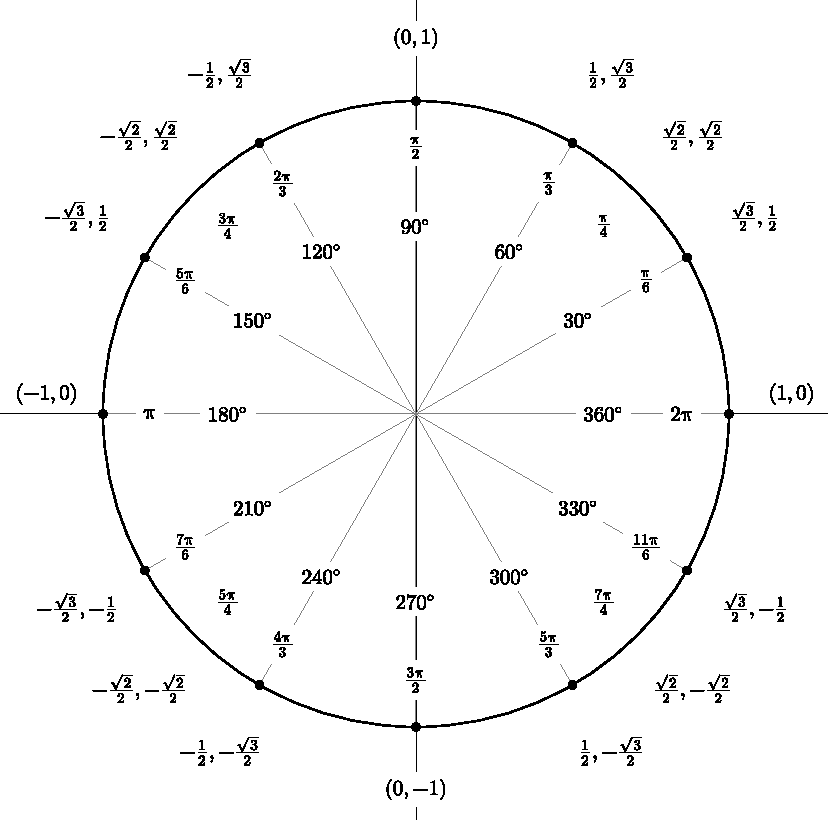
\includegraphics[width=\linewidth]{include_degrees_circle.pdf}
  
\end{center}

\subsubsection*{Taylor expansions 1D at $0$:}
\begin{itemize}
 \item $\sin(x) = \sumn (-1)^n \cdot \frac{x^{2n+1}}{(2n+1)!}$
 \item $\cos(x) = \sumn (-1)^n \cdot \frac{x^{2n}}{(2n)!}$
 \item $e^x = \sumn \frac{x^n}{n!}$
 \item $e^{-x} = \sumn (-1)^n \cdot \frac{x^n}{n!}$
 \item $\sinh(x) = \sumn \frac{x^{2n+1}}{(2n+1)!}$
 \item $\cosh(x) = \sumn \frac{x^{2n}}{(2n)!}$
\end{itemize}


\section{Tables}
\subsection*{Derivations}
\begin{center}
  % the c>{\centering\arraybackslash}X is a workaround to have a column fill up all space and still be centered
  \begin{tabularx}{\linewidth}{c>{\centering\arraybackslash}Xc}
    \toprule
    $\mathbf{F(x)}$ & $\mathbf{f(x)}$ & $\mathbf{f'(x)}$ \\
    \midrule
    $\frac{x^{-a+1}}{-a+1}$ & $\frac{1}{x^a}$ & $\frac{a}{x^{a+1}}$ \\
    $\frac{x^{a+1}}{a+1}$ & $x^a \ (a \ne 1)$ & $a \cdot x^{a-1}$ \\
    $\frac{1}{k \ln(a)}a^{kx}$ & $a^{kx}$ & $ka^{kx} \ln(a)$ \\
    $\ln |x|$ & $\frac{1}{x}$ & $-\frac{1}{x^2}$ \\
    $\frac{2}{3}x^{3/2}$ & $\sqrt{x}$ & $\frac{1}{2\sqrt{x}}$\\
    $-\cos(x)$ & $\sin(x)$ & $\cos(x)$ \\
    $\sin(x)$ & $\cos(x)$ & $-\sin(x)$ \\
    $\frac{1}{2}(x-\frac{1}{2}\sin(2x))$ & $\sin^2(x)$ & $2 \sin(x)\cos(x)$ \\
    $\frac{1}{2}(x + \frac{1}{2}\sin(2x))$ & $\cos^2(x)$ & $-2\sin(x)\cos(x)$ \\
    \multirow{2}*{$-\ln|\cos(x)|$} & \multirow{2}*{$\tan(x)$} & $\frac{1}{\cos^2(x)}$  \\
    & & $1 + \tan^2(x)$ \\
    $\cosh(x)$ & $\sinh(x)$ & $\cosh(x)$ \\
    $\log(\cosh(x))$ & $\tanh(x)$ & $\frac{1}{\cosh^2(x)}$ \\
    $\ln | \sin(x)|$ & $\cot(x)$ & $-\frac{1}{\sin^2(x)}$ \\
    $\frac{1}{c} \cdot e^{cx}$ & $e^{cx}$ & $c \cdot e^{cx}$ \\
    $x(\ln |x| - 1)$ & $\ln |x|$ & $\frac{1}{x}$ \\
    $\frac{1}{2}(\ln(x))^2$ & $\frac{\ln(x)}{x}$ & $\frac{1 - \ln(x)}{x^2}$ \\
    $\frac{x}{\ln(a)} (\ln|x| -1)$ & $\log_a |x|$ & $\frac{1}{\ln(a)x}$ \\
    \bottomrule
  \end{tabularx}
\end{center}
\subsection*{Further derivations}
\begin{center}
  \begin{tabularx}{\linewidth}{>{\centering\arraybackslash}X>{\centering\arraybackslash}X}
    \toprule
    $\mathbf{F(x)}$ & $\mathbf{f(x)}$ \\
    \midrule
    $\arcsin(x)$ & $\frac{1}{\sqrt{1 - x^2}}$ \\
    $\arccos(x)$ & $\frac{-1}{\sqrt{1 - x^2}}$ \\
    $\arctan(x)$ & $\frac{1}{1 + x^2}$ \\ 
    $x^x \ (x > 0)$ & $x^x \cdot (1 + \ln x)$ \\
    \bottomrule
  \end{tabularx}
\end{center}
\subsection*{Integrals}
\begin{center}
  \begin{tabularx}{\linewidth}{>{\centering\arraybackslash}X>{\centering\arraybackslash}X}
    \toprule
    $\mathbf{f(x)}$ & $\mathbf{F(x)}$ \\
    \midrule
    $\int f'(x) f(x) \dx$ & $\frac{1}{2}(f(x))^2$ \\
    $\int \frac{f'(x)}{f(x)} \dx$ & $\ln|f(x)|$ \\
    $\int_{-\infty}^\infty e^{-x^2} \dx$ & $\sqrt{\pi}$ \\
    $\int (ax+b)^n \dx$ & $\frac{1}{a(n+1)}(ax+b)^{n+1}$ \\
    $\int x(ax+b)^n \dx$ & $\frac{(ax+b)^{n+2}}{(n+2)a^2} - \frac{b(ax+b)^{n+1}}{(n+1)a^2}$ \\
    $\int (ax^p+b)^n x^{p-1} \dx$ & $\frac{(ax^p+b)^{n+1}}{ap(n+1)}$ \\
    $\int (ax^p + b)^{-1} x^{p-1} \dx$ & $\frac{1}{ap} \ln |ax^p + b|$ \\
    $\int \frac{ax+b}{cx+d} \dx$ & $\frac{ax}{c} - \frac{ad-bc}{c^2} \ln |cx +d|$ \\
    $\int \frac{1}{x^2+a^2} \dx$ & $\frac{1}{a} \arctan \frac{x}{a}$ \\
    $\int \frac{1}{x^2 - a^2} \dx$ & $\frac{1}{2a} \ln\left| \frac{x-a}{x+a} \right|$ \\
    $\int \sqrt{a^2+x^2} \dx $ & $\frac{x}{2}f(x) + \frac{a^2}{2}\ln(x+f(x))$ \\
    \bottomrule
  \end{tabularx}
\end{center}

% end of larger array spacing
\endgroup
\section{Sources}
This cheatsheet was inspired by previous summaries from Julian (xyquadrat) and Nicolas(Franco). 

Apart from that the definitions were taken from the ``Analysis 2'' script by E. Kowalski and the Lecture Notes from Ö. Imamoglu in the HS2022 edition of the course.
\end{document}